\Subsection{Definition}

Consider an array $a[1..n]$. Its elements form a binary tree with a root at $1$.

Children of a vertex at $i$ are vertices at $2i$ and $2i+1$; the parent of a vertex at $i$ is $\lfloor \frac{i}{2} \rfloor$.

\begin{definition}\textbf{Binary heap}

    A binary heap is an array indicies of which form the described above tree which in turn holds the following property: $\forall$ vertex $i$ the value $a[i]$ is a \textbf{minimum} in a subtree of $i$.

    \begin{center}
        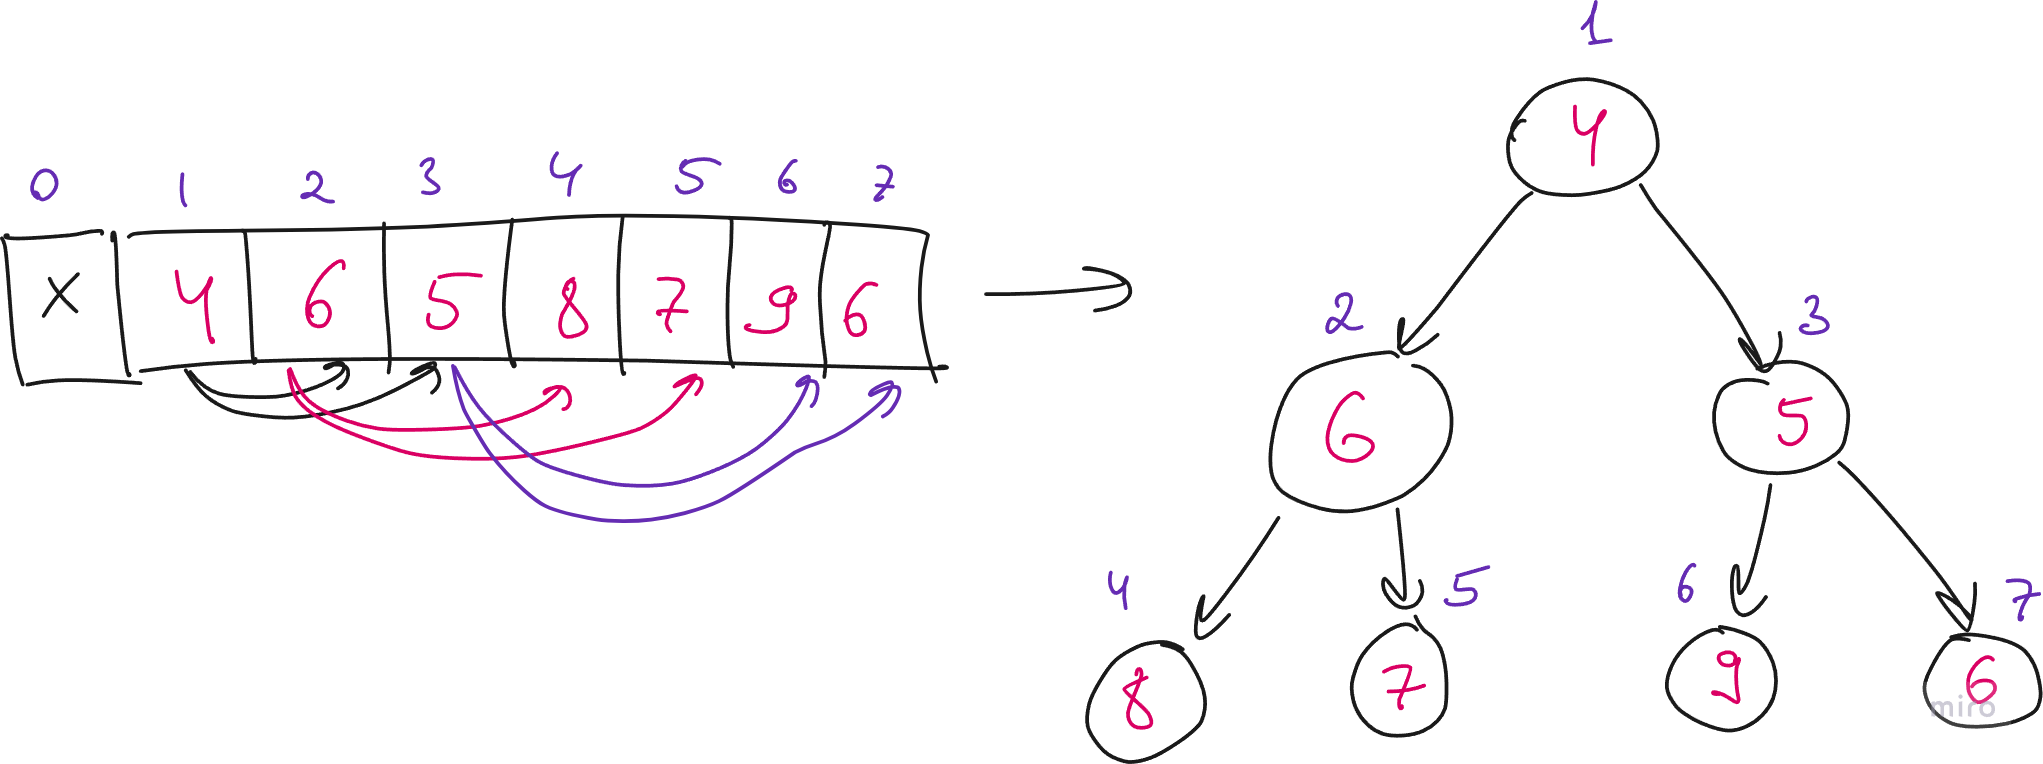
\includegraphics[scale=0.25]{./assets/12-binary-heap/1.png}
    \end{center}

\end{definition}

\begin{lemma}

    The height of the binary heap is $\lfloor \log_{2}{n} \rfloor$.

\end{lemma}

\begin{proof}

    The height is equal to the length of the distance between the vertex at $n$ and the root at $1$. Notice, that by the definition $\forall k$: distance from the root to vertices from the range $[2^k, 2^{k+1})$ is equal to $k$ $\implies$ for the vertex at $n$ its corresponding $k := \lfloor \log_{2}{n} \rfloor$ (it is a simple induction over $k$):

    Let $d_{k}$ be the distance between (in terms of the number of edges) the root and the vertices from the range $[2^k, 2^{k+1})$. We want to prove $d_{k} \equiv k$:

    1. \textbf{Base}: $k=1$

    $[2^1, 2^{2}) = [2, 2^2-1] = [2, 3]$ - distance $d_{1}$ between the root and vertices $2$ and $3$ is indeed $1$ by the definition, thus $d_{1} = k$.

    2. \textbf{Transition:} $k \to k+1$:

    Let's consider the range on the step $k$: $[2^k, 2^{k+1}-1]$, now let's see what are the children for the vertex $v_1 = 2^k$ and the vertex $v_2 = 2^{k+1}-1$ (children of all vertices between $v_1$ and $v_2$ will have numbers in between the obtained range):

        1. $v_1$: $2^k \to 2^{k+1}, 2^{k+1}-1$.

        2. $v_2$: $2^{k+1}-1 \to 2^{k+2}-2, 2^{k+2}-1$.

        Thus, the obtained range will be $[2^{k+1}, 2^{k+2}-1]$, i.e. the distance $d_{k+1}$ from the root to the vertices in this range will be $d_{k+1} = d_{k} + 1 = k+1 \implies d_{k+1} = k+1$.

\end{proof}

\textbf{Interface}:

The binary heap due to its height executes in $O(\log{n})$ the following operations:

1. $GetMin()$ - find the minimum element (works in $O(1)$).

2. $Add(x)$ - add a new element.

3. $ExtractMin()$ - remove the current minimum element.

If there is a support of \textit{reversed references} which allow access to the position $i$ by a given element $a[i]$ in $O(1)$, then the binary heap will also support the following operations:

1. $DecreaseKey(x, c)$ - decrease a value $x$ by $c$.

2. $Del(x)$ - remove element $x$ from the heap.

\Subsection{siftUp, siftDown}

\textbf{siftUp(i)} - push up (bubble up) an element at the position $i$.

\textbf{siftDown(i)} - push down an element at the position $i$.

Both operations require the heap to comply with its definition for all position except the position $i$, i.e. these operations place an element at the position $i$ into such a position, so that the underlying property of a heap starts to hold for all elements.

\begin{lstlisting}[language=C++]
void siftUp(int i) {
    int p = i / 2;
    // while i is not a root and parent's value is greater than value of i
    while (i > 1 && a[p] > a[i]) {
        swap(a[i], a[p]);
        i /= 2;
    }
}

void siftDown(int i) {
    while (true) {
        int l = 2 * i;
        // select a smaller child of i
        if (l + 1 <= n && a[l + 1] < a[l]) ++l;
        // if both children are not less than i
        if (l > n || a[l] >= a[i]) break;
        // go to the child
        swap(a[l], a[i]);
        i = l;
    }
}
\end{lstlisting}

\begin{lemma}

    Both operations work in $O(\log{n})$.

\end{lemma}

\begin{proof}

    Both operations work in $O(\text{heap height}) = O(\log{n})$.

\end{proof}



\Subsection{GetMin, Add, ExtractMin}

All of these operations can be expressed via \textbf{siftUp}/\textbf{siftDown}.

\begin{lstlisting}[language=C++]
vector<int> h(N + 1);
int n = 0; // current size (i.e. the number of elements)

int GetMin() {
    return a[1];
}

void Add(int x) {
    ++n;
    a[n] = x;
    siftUp(n);
}

void ExtractMin() {
    // extracting root
    swap(a[1], a[n]);
    n--;
    siftDown(1);
}
\end{lstlisting}

Example of the \textbf{siftUp} operation during \textbf{Add}:

\begin{center}
    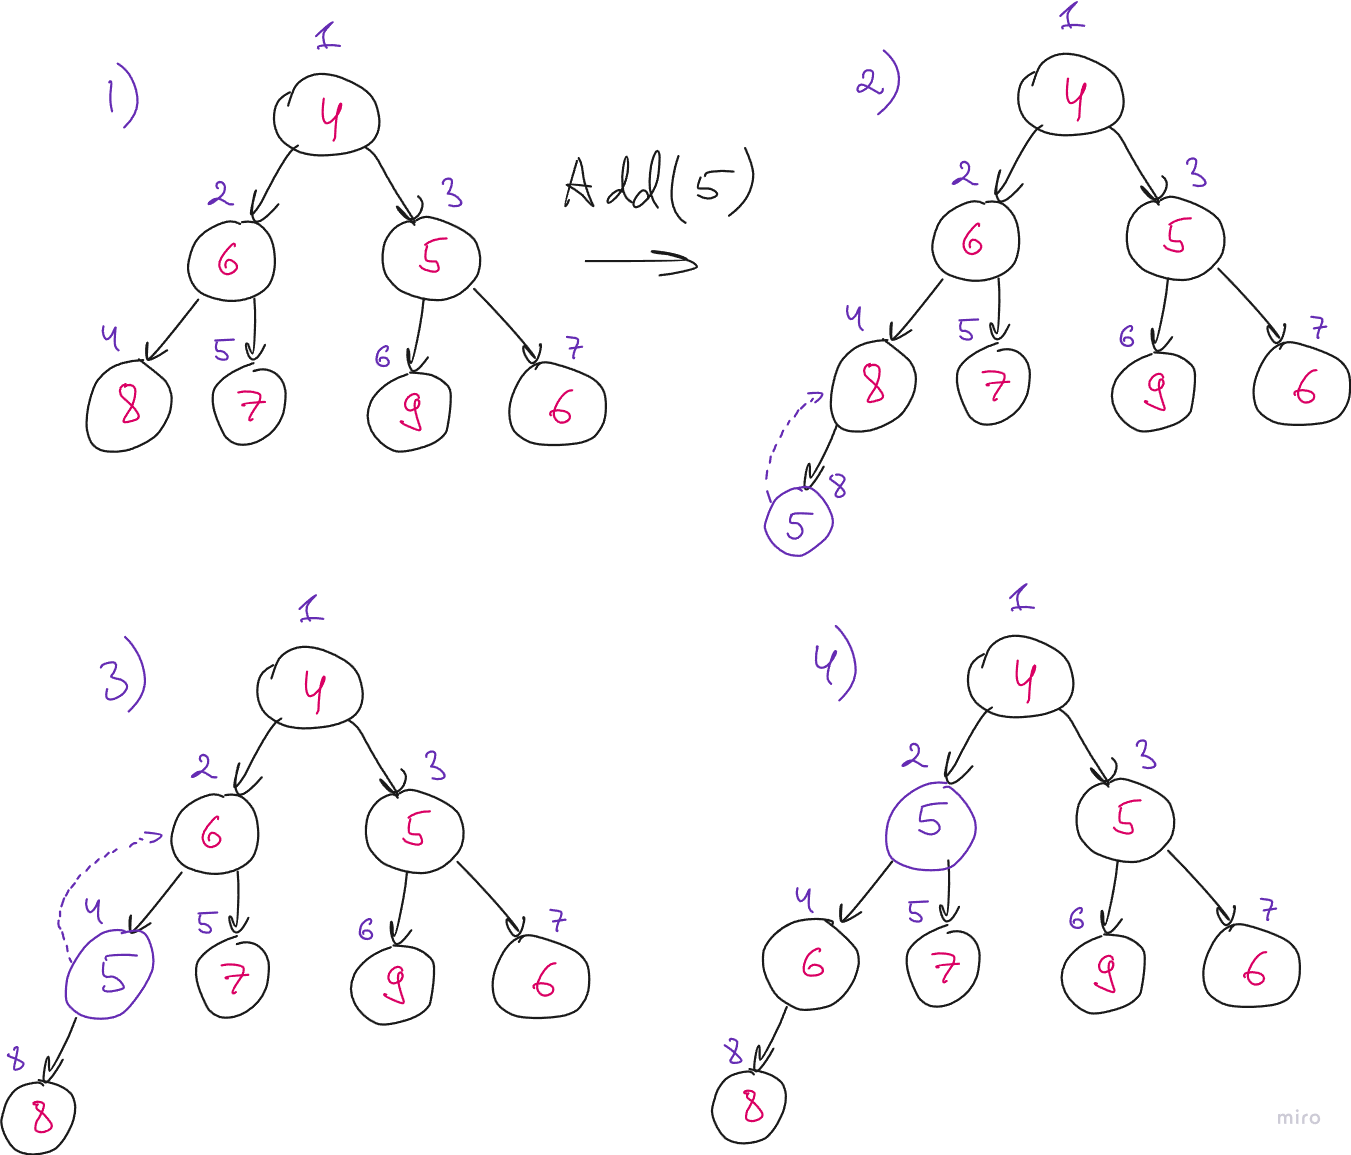
\includegraphics[scale=0.25]{./assets/12-binary-heap/4.png}
\end{center}

Example of the \textbf{siftDown} operation during \textbf{ExtractMin}:

\begin{center}
    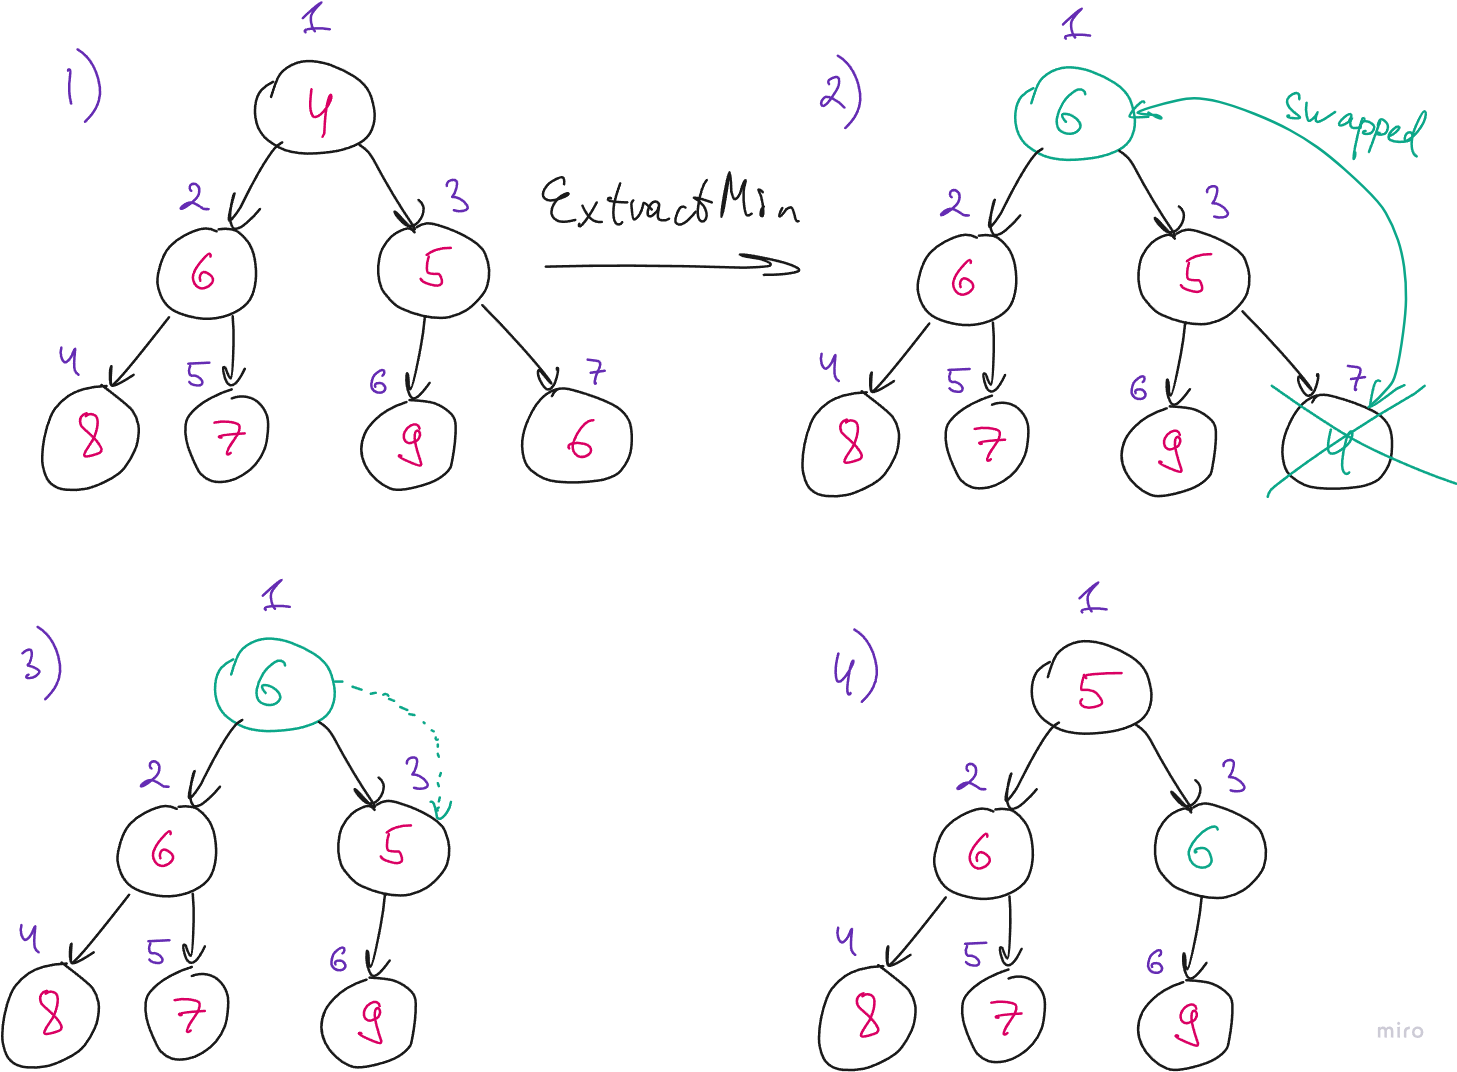
\includegraphics[scale=0.25]{./assets/12-binary-heap/5.png}
\end{center}


\Subsection{Reversed references and DecreaseKey}

Suppose now we have an array \textbf{vector<int> values}. In the heap \textbf{a[]} we will store indicies of the array \textbf{values}. In this case all comparisons $a[i] < a[j]$ will be rewritten as $\text{values}[a[i]] < \text{values}[a[j]]$. In order to add an element we need to add it inside \textbf{values}: \textbf{values.push\_back(x)} and then add its index inside the heap: \textbf{Add(values.size() - 1)}. Since now we store the indicies inside the heap, we can for every $i$ store an index inside the heap, i.e. \textbf{pos[i]} = position of the $i$-th element of \textbf{values} in \textbf{a}.

1. Given position in the heap $\to$ get its value: $i \to a[i] \to \text{values}[a[i]]$.

2. Property of \textbf{pos}: $i \to \text{pos}[i] \to a[\text{pos}[i]] = i$.

The values of \textbf{pos[]} must be recalculated every time when we modify \textbf{a[]}.

See the following image for clarifications:

\begin{center}
    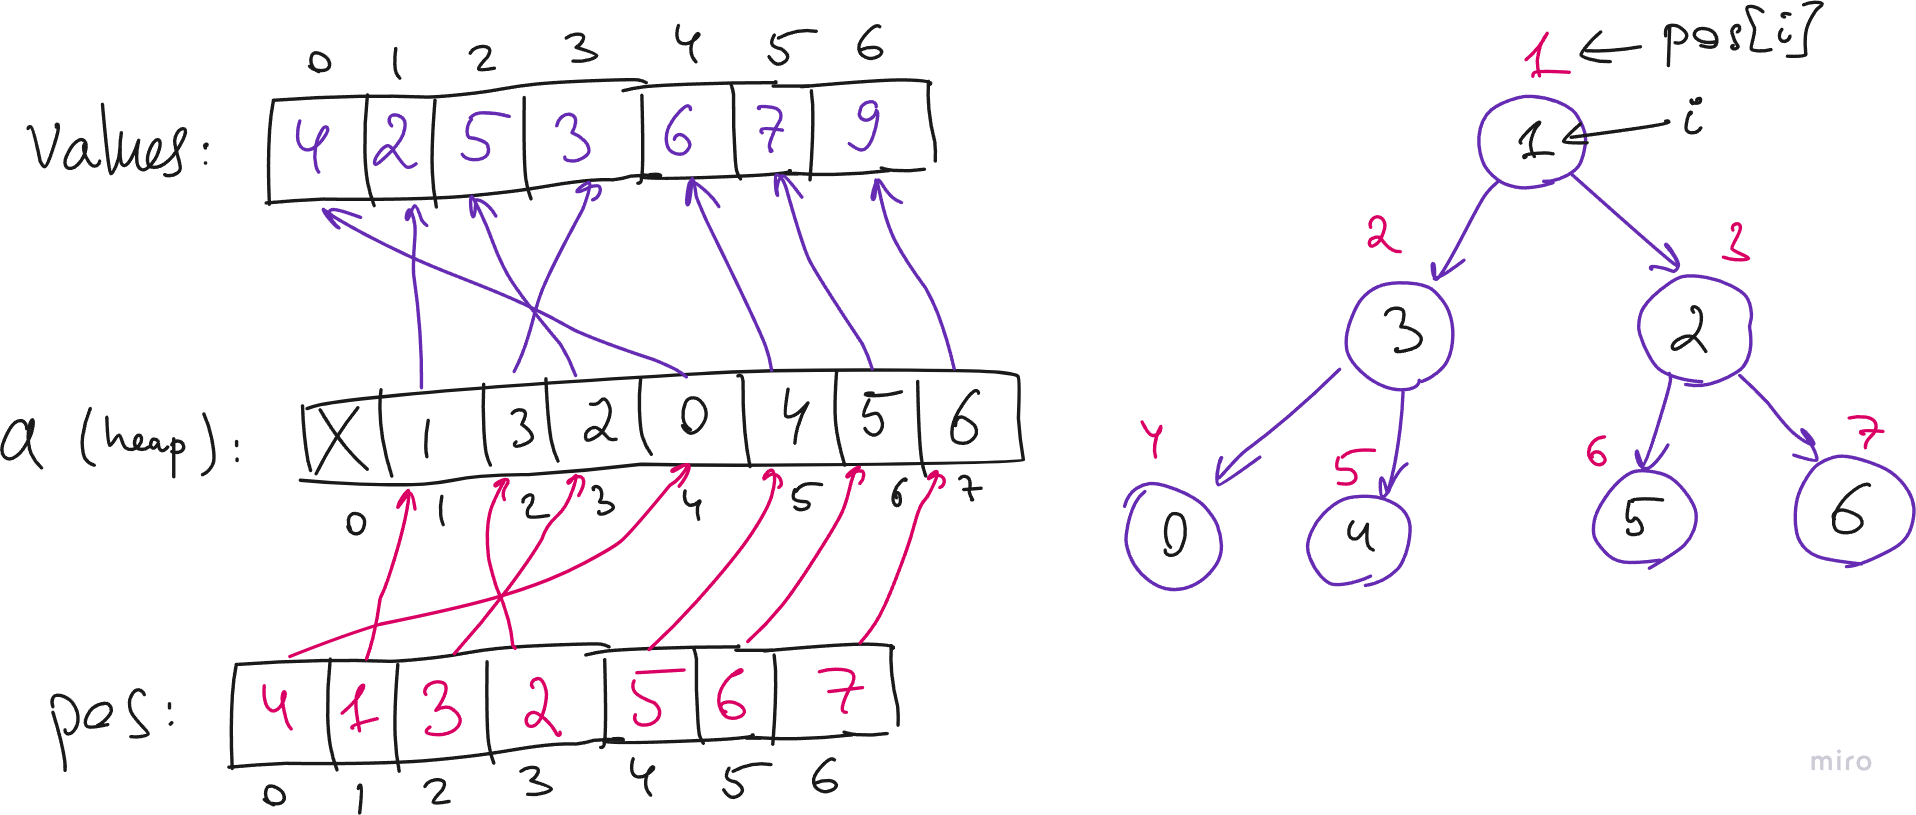
\includegraphics[scale=0.25]{./assets/12-binary-heap/3.png}
\end{center}

Now we can implement removal and decrease of a key of an element inside \textbf{values} by its index $i$ in $O(\log{n})$ of time:

\begin{lstlisting}[language=C++]
void Del(int i) {
    // i - index inside values[]
    int ind = pos[i]; // index inside heap a[]

    a[ind] = h[n]; n--;
    pos[a[ind]] = ind; // update pos[] for the 'a[ind]'-th element of values[]

    // both sift operations because new element can be
    // either greater than its children or less than its parent
    siftUp(ind);
    siftDown(ind);
}

void DecreaseKey(int i, int c) {
    // i - index inside values
    values[i] -= c;
    int ind = pos[i]; // index inside heap a[]

    // the updated element could become less than its parent
    siftUp(ind);
}
\end{lstlisting}


\Subsection{Build, HeapSort}

We can construct a heap from a list of given elements inplace:

\begin{lstlisting}[language=C++]
void Build(int n, int a[]) {
    for (int i = n; i >= 1; --i) {
        siftDown(i);
    }
}
\end{lstlisting}

\begin{lemma}
    The \textbf{Build} operation will construct a correct binary heap from the array \textbf{a[]}.
\end{lemma}

\begin{proof}
    When we push down $i$, due to induction assumption, the left and the right subtrees are already correct binary heaps. Due to correctness of \textbf{siftDown} operation after its execution the subtree at $i$ will become a correct binary heap.
\end{proof}

\begin{lemma}
    \textbf{Build} works in $\Theta(n)$ of time.
\end{lemma}

\begin{proof}
    Let $n = 2^k-1$, then our heap is a full binary tree, because each element except for the leaves will have 2 children. The last level of the heap will contain $2^{k-1}$ elements, the pre-last level will contain $2^{k-2}$ elements, and so on.

    \textbf{siftDown(i)} works in $O(\text{depth of the subtree of $i$})$, thus its total time will be:

    $\sum_{i=1}^{k} 2^{k-i} \cdot i = 2^k \cdot \sum_{i=1}^{k} \frac{i}{2^i} =_{(*)} 2^k \cdot \Theta(1) = (n+1) \cdot \Theta(1) = \Theta(n)$.

    (*): Need to proof that $\sum_{i=1}^{k} \frac{i}{2^i} = \textbf{const}$;

    Notice that $\sum_{i=1}^{k} \frac{i}{2^i} = 2 - \frac{k+2}{2^k}$ (I used \href{https://www.wolframalpha.com/}{wolframalpha} :)). Let's prove it via induction:

    1. \textbf{Base}: $k=1$:

    $\sum_{i=1}^{k} \frac{i}{2^i} = \frac{1}{2} = 2 - \frac{3}{2}$ - the assumption holds.

    2. \textbf{Transition}: $k \to k+1$:

    $\sum_{i=1}^{k+1} \frac{i}{2^i} = \sum_{i=1}^{k} \frac{i}{2^i} + \frac{k+1}{2^{k+1}} = 2 - \frac{k+2}{2^k} + \frac{k+1}{2^{k+1}} = 2 - \frac{k+3}{2^{k+1}} = 2 - \frac{(k+1)+2}{2^{k+1}}$.

\end{proof}

The \textbf{HeapSort} implementation that works in $O(n \log{n})$ and uses $O(1)$ of additional memory due to \textbf{Build} working inplace:

\begin{lstlisting}[language=C++]
void HeapSort(int n, int a[]) {
    Build(n, a);

    for(int i = 0; i < n; ++i) {
        // extracting values in ascending order
        int x = GetMin();
        ExtractMin();
    }
}
\end{lstlisting}
